68. Выразим $x:\ x=2y+4.$ Тогда $(2y+4)^2-2(2y+4)y+8y^2=4y^2+16y+16-4y^2-8y+8y^2=8y^2+8y+16=8(y^2+y+2)=8\left(\left(y+\cfrac{1}{2}\right)^2+\cfrac{7}{4}\right)\geqslant8\cdot\cfrac{7}{4}=14.$\newpage
\noindent69. Для нахождения области определения функции необходимо решить неравенство $\cfrac{x^2+8x+15}{x-2}\geqslant0\Leftrightarrow
\cfrac{(x+3)(x+5)}{x-2}\geqslant0.$ Применив метод интервалов, найдём ответ:
\begin{figure}[ht!]
\center{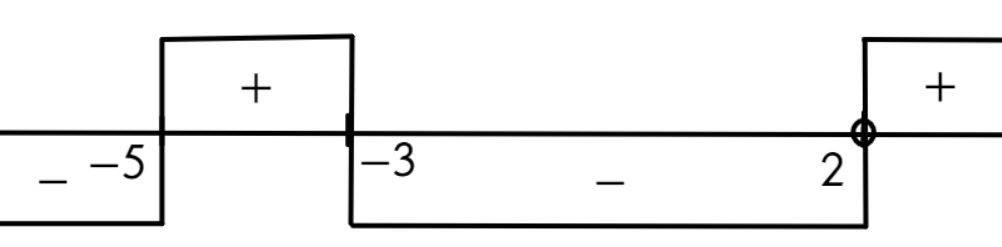
\includegraphics[scale=0.35]{isl69.png}}
\end{figure}
$x\in[-5;-3]\cup(2;+\infty).$\\
